\subsection{bpmprocess/ddc\_\-sample\_\-waveform.c File Reference}
\label{ddc__sample__waveform_8c}\index{bpmprocess/ddc\_\-sample\_\-waveform.c@{bpmprocess/ddc\_\-sample\_\-waveform.c}}


\subsubsection{Detailed Description}


Definition in file {\bf ddc\_\-sample\_\-waveform.c}.

{\tt \#include $<$stdio.h$>$}\par
{\tt \#include $<$stdlib.h$>$}\par
{\tt \#include $<$bpm/bpm\_\-units.h$>$}\par
{\tt \#include $<$bpm/bpm\_\-messages.h$>$}\par
{\tt \#include $<$bpm/bpm\_\-process.h$>$}\par


Include dependency graph for ddc\_\-sample\_\-waveform.c:\nopagebreak
\begin{figure}[H]
\begin{center}
\leavevmode
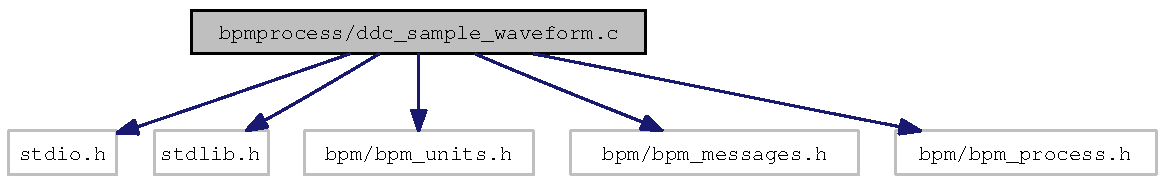
\includegraphics[width=297pt]{ddc__sample__waveform_8c__incl}
\end{center}
\end{figure}
\subsubsection*{Functions}
\begin{CompactItemize}
\item 
int {\bf ddc\_\-sample\_\-waveform} ({\bf doublewf\_\-t} $\ast$w, double frequency, {\bf filter\_\-t} $\ast$filt, int iSample, double t0, double tdecay, double $\ast$amp, double $\ast$phase, {\bf doublewf\_\-t} $\ast$buf\_\-re, {\bf doublewf\_\-t} $\ast$buf\_\-im)
\end{CompactItemize}
